\documentclass[mstat,12pt]{unswthesis}


\usepackage{pgfgantt}

%%%%%%%%%%%%%%%%%%%%%%%%%%%%%%%%%%%%%%%%%%%%%%%%%%%%%%%%%%%%%%%%%%
% 
% OK...Now we get to some actual input.  The first part sets up
% the title etc that will appear on the front page
%
%%%%%%%%%%%%%%%%%%%%%%%%%%%%%%%%%%%%%%%%%%%%%%%%%%%%%%%%%%%%%%%%%

\title{Group Project Plan by Team What Watts\\[0.5cm]A Data Science
Approach to Forecast Electricity Consumption in Australia}

\authornameonly{(Nee) Jittinun Trairattanasirikul - (z5281789) (Ruhul)
Md Ruhul Amin Sarker - (z5275314) Peter Morian - (z5017159) James
Cleaver - (z5283034) }

\author{\Authornameonly}

\copyrightfalse
\figurespagefalse
\tablespagefalse

%%%%%%%%%%%%%%%%%%%%%%%%%%%%%%%%%%%%%%%%%%%%%%%%%%%%%%%%%%%%%%%%%
%
%  And now the document begins
%  The \beforepreface and \afterpreface commands puts the
%  contents page etc in
%
%%%%%%%%%%%%%%%%%%%%%%%%%%%%%%%%%%%%%%%%%%%%%%%%%%%%%%%%%%%%%%%%%%


%%%%%%%%%%%%%%%%%%%%%%%%%%%%%%%%%%%%%%%%%%%%%%%%%%%%%%%%%%%%%%%%%%%%%%%
%
%  A small sample UNSW Coursework Masters thesis file.
%  Any questions to Ian Doust i.doust@unsw.edu.au and/or Gery Geenens ggeenens@unsw.edu.au
%
%%%%%%%%%%%%%%%%%%%%%%%%%%%%%%%%%%%%%%%%%%%%%%%%%%%%%%%%%%%%%%%%%%%%%%%
%
%  The first part pulls in a UNSW Thesis class file.  This one is
%  slightly nonstandard and has been set up to do a couple of
%  things automatically
%
 
%%%%%%%%%%%%%%%%%
%% Precisely one of the next four lines should be uncommented.
%% Choose the one which matches your degree, uncomment it, and comment out the other two!
%\documentclass[mfin,12pt]{unswthesis}    %%  For Master of Financial Mathematics 
%\documentclass[mmath,12pt]{unswthesis}   %%  For Master of Mathematics
%\documentclass[mstat,12pt]{unswthesis}  %%  For Master of Statistics
%%%%%%%%%%%%%%%%%



\linespread{1}
\usepackage{amsfonts}
\usepackage{amssymb}
\usepackage{amsthm}
\usepackage{latexsym,amsmath}
\usepackage{graphicx}
\usepackage{afterpage}
\usepackage[colorlinks]{hyperref}
 \hypersetup{
     colorlinks=true,
     linkcolor=blue,
     filecolor=blue,
     citecolor= black,      
     urlcolor=cyan,
     }
\usepackage{textcomp}
\usepackage{longtable}
\usepackage{booktabs}
\usepackage{float}

%%%%%%%%%%%%%%%%%%%%%%%%%%%%%%%%%%%%%%%%%%%%%%%%%%%%%%%%%%%%%%%%%
%
%  The following are some simple LaTeX macros to give some
%  commonly used letters in funny fonts. You may need more or less of
%  these
%
\newcommand{\R}{\mathbb{R}}
\newcommand{\Q}{\mathbb{Q}}
\newcommand{\C}{\mathbb{C}}
\newcommand{\N}{\mathbb{N}}
\newcommand{\F}{\mathbb{F}}
\newcommand{\PP}{\mathbb{P}}
\newcommand{\T}{\mathbb{T}}
\newcommand{\Z}{\mathbb{Z}}
\newcommand{\B}{\mathfrak{B}}
\newcommand{\BB}{\mathcal{B}}
\newcommand{\M}{\mathfrak{M}}
\newcommand{\X}{\mathfrak{X}}
\newcommand{\Y}{\mathfrak{Y}}
\newcommand{\CC}{\mathcal{C}}
\newcommand{\E}{\mathbb{E}}
\newcommand{\cP}{\mathcal{P}}
\newcommand{\cS}{\mathcal{S}}
\newcommand{\A}{\mathcal{A}}
\newcommand{\ZZ}{\mathcal{Z}}
%%%%%%%%%%%%%%%%%%%%%%%%%%%%%%%%%%%%%%%%%%%%%%%%%%%%%%%%%%%%%%%%%%%%%
%
% The following are much more esoteric commands that I have left in
% so that this file still processes. Use or delete as you see fit
%
\newcommand{\bv}[1]{\mbox{BV($#1$)}}
\newcommand{\comb}[2]{\left(\!\!\!\begin{array}{c}#1\\#2\end{array}\!\!\!\right)
}
\newcommand{\Lat}{{\rm Lat}}
\newcommand{\var}{\mathop{\rm var}}
\newcommand{\Pt}{{\mathcal P}}
\def\tr(#1){{\rm trace}(#1)}
\def\Exp(#1){{\mathbb E}(#1)}
\def\Exps(#1){{\mathbb E}\sparen(#1)}
\newcommand{\floor}[1]{\left\lfloor #1 \right\rfloor}
\newcommand{\ceil}[1]{\left\lceil #1 \right\rceil}
\newcommand{\hatt}[1]{\widehat #1}
\newcommand{\modeq}[3]{#1 \equiv #2 \,(\text{mod}\, #3)}
\newcommand{\rmod}{\,\mathrm{mod}\,}
\newcommand{\p}{\hphantom{+}}
\newcommand{\vect}[1]{\mbox{\boldmath $ #1 $}}
\newcommand{\reff}[2]{\ref{#1}.\ref{#2}}
\newcommand{\psum}[2]{\sum_{#1}^{#2}\!\!\!'\,\,}
\newcommand{\bin}[2]{\left( \begin{array}{@{}c@{}}
				#1 \\ #2
			\end{array}\right)	}
%
%  Macros - some of these are in plain TeX (gasp!)
%
\newcommand{\be}{($\beta$)}
\newcommand{\eqp}{\mathrel{{=}_p}}
\newcommand{\ltp}{\mathrel{{\prec}_p}}
\newcommand{\lep}{\mathrel{{\preceq}_p}}
\def\brack#1{\left \{ #1 \right \}}
\def\bul{$\bullet$\ }
\def\cl{{\rm cl}}
\let\del=\partial
\def\enditem{\par\smallskip\noindent}
\def\implies{\Rightarrow}
\def\inpr#1,#2{\t \hbox{\langle #1 , #2 \rangle} \t}
\def\ip<#1,#2>{\langle #1,#2 \rangle}
\def\lp{\ell^p}
\def\maxb#1{\max \brack{#1}}
\def\minb#1{\min \brack{#1}}
\def\mod#1{\left \vert #1 \right \vert}
\def\norm#1{\left \Vert #1 \right \Vert}
\def\paren(#1){\left( #1 \right)}
\def\qed{\hfill \hbox{$\Box$} \smallskip}
\def\sbrack#1{\Bigl \{ #1 \Bigr \} }
\def\ssbrack#1{ \{ #1 \} }
\def\smod#1{\Bigl \vert #1 \Bigr \vert}
\def\smmod#1{\bigl \vert #1 \bigr \vert}
\def\ssmod#1{\vert #1 \vert}
\def\sspmod#1{\vert\, #1 \, \vert}
\def\snorm#1{\Bigl \Vert #1 \Bigr \Vert}
\def\ssnorm#1{\Vert #1 \Vert}
\def\sparen(#1){\Bigl ( #1 \Bigr )}

\newcommand\blankpage{%
    \null
    \thispagestyle{empty}%
    \addtocounter{page}{-1}%
    \newpage}

%%%%%%%%%%%%%%%%%%%%%%%%%%%%%%%
%
% These environments allow you to get nice numbered headings
%  for your Theorems, Definitions etc.  
%
%  Environments
%
%%%%%%%%%%%%%%%%%%%%%%%%%%%%%%%

\newtheorem{theorem}{Theorem}[section]
\newtheorem{lemma}[theorem]{Lemma}
\newtheorem{proposition}[theorem]{Proposition}
\newtheorem{corollary}[theorem]{Corollary}
\newtheorem{conjecture}[theorem]{Conjecture}
\newtheorem{definition}[theorem]{Definition}
\newtheorem{example}[theorem]{Example}
\newtheorem{remark}[theorem]{Remark}
\newtheorem{question}[theorem]{Question}
\newtheorem{notation}[theorem]{Notation}
\numberwithin{equation}{section}

%%%%%%%%%%%%%%%%%%%%%%%%%%%%%%%%%%%%%%%%%%%%%%%%%%%%%%%%%%%%%%%%%%
%
%  If you've got some funny special words that LaTeX might not
% hyphenate properly, you can give it a helping hand:
%

\hyphenation{Mar-cin-kie-wicz Rade-macher}






\begin{document}

\beforepreface

\prefacesection{Abstract}

The increase of Rooftop Solar in NSW has changed the energy supply and
demand model and forecasts. We aim to improve the quality of the
existing forecasting done by the Australian Energy Market Operator
(AEMO). Through this project we will use the existing forecast data as
well as additional solar information to improve the accuracy of the
current forecast demand. We will use RMSE as the metric to show
improvement against the forecast and total demand data since 2010.

%\afterpage{\blankpage}


\afterpreface





%%%%%%%%%%%%%%%%%%%%%%%%%%%%%%%%%%%%%%%%%%%%%%%%%%%%%%%%%%%%%%%%%%
%
% Now we can start on the first chapter
% Within chapters we have sections, subsections and so forth
%
%%%%%%%%%%%%%%%%%%%%%%%%%%%%%%%%%%%%%%%%%%%%%%%%%%%%%%%%%%%%%%%%%%



%%%%%%%%%%%%%%%%%%%%%%%%%%%%%%%%%%%%%

%\afterpage{\blankpage}


\setcounter{chapter}{1}
\renewcommand\thesection{\arabic{section}}

\hypertarget{introduction-and-motivation}{%
\section{Introduction and
Motivation}\label{introduction-and-motivation}}

We aim to create a model that can predict the demand for electricity to
a higher degree of accuracy that the current methods used for
forecasting demand. We believe that the gap between forecasted and true
demand is partly explained by accounting for solar panels and their
usage throughout the day. Thus using temperature data, as well as other
external datasets such as solar data. We intend on using a Neural
Network to fill-in the gaps between the current forecasted and true
demand. Given that the current RMSE between forecasted and true
electricity demand is roughly 85.87, the measure of success for this
project is to build a more accurate model with an RMSE of at most 75. By
taking into account solar panel usage, we intend on building a model
that can predict electricity demand with more certainty.

\hypertarget{brief-literature-review}{%
\section{Brief Literature Review}\label{brief-literature-review}}

Since 1998 the East Coast Australian Energy Market has been driven by
the National Energy Market (NEM). This is an organisation that since
2005 has rules set by the Australian Energy Market Commission (AEMC) and
since 2009 the operational day to day management of the NEM has been
managed by Australian Energy Market Operator (AEMO). The NEM is
accountable for matching the supply and demand of the Electricity
market, it does this through 2 main mechanisms, a spot market that
ensures electricity in real time, and sends signals to the electricity
suppliers to power up and down generators, and contract market that
provides surety in electrical supply in the long term. Roof top solar
has been on the increase form 0.2\% od houses in 2007 upto 20\% of
houses in 2020. This increase is expected to continue with the AEMO
predicting that by 2030 up to 30000MW of electricity will be generated
by Solar \cite{aemo_2020_projections} and is expected to be one of the
largest impacts to energy demand, Roof top solar provides individual
houses with their electricity needs during high solar periods, as such
they are not putting load on the grid \cite{parkinson_2019_rooftop} .
The current forecast models that are created by the AEMO do not include
the rooftop solar as part of their demand, as it is not required to be
included in either the contract or spot markets.Whilst Modeling has been
done in other locations that include rooftop solar, it has not been
included in the NEM data todate \cite{aemo_electicity}. Techniques such
as linear regressions, neural networks have been used to model Energy
Demand Data in the past\cite{marcjasz_2008_neural}, however to date the
inclusion of solar information has not been included in the NSW
modeling\cite{nem_2021_mms}. Our investigation intends to use either
synthetic solar information based on the bankstown latitude and
longitude as being representative of the solar profile of NSW (based on
the current population density of people in NSW). This data would then
be used to increase the accuracy of the current AEMO predicted demand
calculations, providing a more accurate RMSE.

\hypertarget{methods-software-and-data-description}{%
\section{Methods, Software and Data
Description}\label{methods-software-and-data-description}}

In terms of the data, we intend on using solar data, NSW Public Holiday
data, temperature, forecast and total demaind electricity datasets and
potentially cloud and wind speed data. Whilst we are aware that getting
more accurate measurements of wind \& cloud coverage will require much
greater granularity and that these features do significantly change over
a geographical area, this level of granular data would also require
collecting information about the locations of rooftop solar panels,
which is not possible. Thus, we are making the assumption that the
external datasets reflect the true wind \& cloud coverage rates of a
region at a given point in time. As 90\% of the population is located
near Sydney we have used the climate zone information based on this
region\cite{abcb_2015_climate}.

For this project, we plan on using Python as the main language for data
preparation, analysis and modelling. Python was selected over R due to
the common familiarity amongst the entire team, and it is well
established amongst the Data Science community that Python is the
language-of-choice for machine learning. For our presentation, we intend
on using Powerpoint, a Google collab notebook, and a Rshiny/Power BI
dashboard for interactive analysis.

Neural Networks are known to handle noisy data well compared to other
models, and given the noisy nature of the electricity demand \&
temperature data, this seems appropriate to use a Neural Network for
modelling. Additionally, since electricity demand \& temperature data
appears to have some form of seasonality, we would like to build a model
that can capture patterns in the data, which would be possible with
Neural Networks. As the data is time-based, we are inclined to use an
LSTM or GRU form of a Neural Network (both will be built \& tested), as
these models retain information from the past when predicting future
values.

\hypertarget{activities-and-schedule}{%
\section{Activities and Schedule}\label{activities-and-schedule}}

Our Project team has chosen to use an agile methodology for managing the
project, for this we are using the Jira tool. Due to the nature of the
team members schedules, and geographical dispersion, the work is being
managed via a wall of work with all team members ``pulling'' work as
they are able. To ensure that the work is being completed the team has
daily communications via whatsapp in the form of a daily standup, with a
Wednesday night checkpoint meeting, and a Saturday sprint planning and
retrospective.

Due to the aggressive timeframe of the project the work has been
structured as a single epic, with larger components being managed as a
story but the majority of the elements being managed as tasks.

We have chosen to load many of the tasks into the initial sprint, while
recognising that the majority of this will spill over into future
sprints. The Scrum manager role is being performed by Nee, however, this
is likely to rotate based on individuals workloads throughout the
project. The Project lead role is being perfomed by James. Peter is
focusing on the development of the neural network model, and Ruhul is
leading the visualisations. The pull nature of the agile mentodology
means all team members will be involved with most tasks.

Task allocation is often being priotised for people wanting to learn the
skills, with people with the current skills acting as reviewers, for
instance James is performing the Rmarkdown to gain the skills whereas
Peter is reviewing as he already has the skills. This way we ensure the
team is able to provide backup for each other throughout the project.

The following table highlights the sprints and due date of the tasks.

\newpage

\begin{figure}
\centering
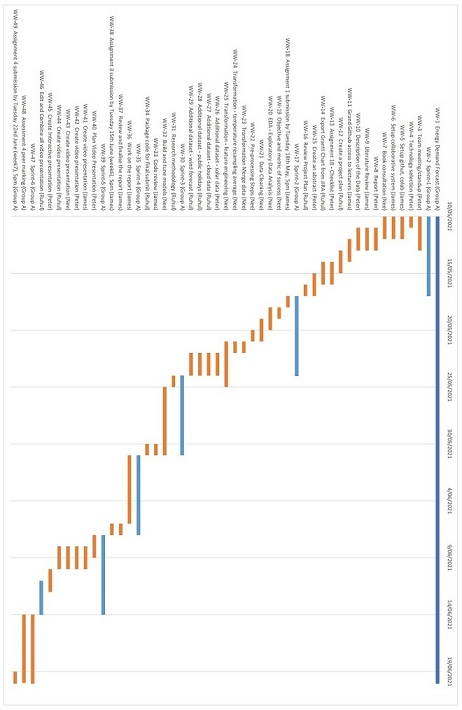
\includegraphics{Gannt.jpg}
\caption{Gannt Chart}
\end{figure}

\bibliographystyle{elsarticle-num}
\bibliography{references}







\end{document}

